\documentclass[journal,twoside,web]{ieeecolor}
\usepackage{jsen}
\usepackage{cite}
\usepackage{amsmath,amssymb,amsfonts}
\usepackage{algorithmic}
\usepackage{graphicx}
\usepackage{textcomp}
\usepackage{wrapfig}
\def\BibTeX{{\rm B\kern-.05em{\sc i\kern-.025em b}\kern-.08em
    T\kern-.1667em\lower.7ex\hbox{E}\kern-.125emX}}
\markboth{Progress Report}
{Author: Joseph Joy \MakeLowercase{\textit{et al.}}: MSc Cyber Security (February 2020)}
\begin{document}
\title{Attacks on Machine Learning}
\author{Joseph Joy, MSc Cyber Security, L00151362
}

\IEEEtitleabstractindextext{\

\begin{abstract}
Machine Learning has been paving the way for other sides of our modern existence. Many systems in which we communicate have a form of Machine Learning to empower them. It covers internet shopping, social networking, voice guides, childcare, and banking. Although it is irrefutable to conclude that Machine Learning has improved computing system capacities, it is worth addressing the bugs and security issues that exist in applications that exploit this technology as well. Adversarial Assaults, data poisoning, and model stealing techniques are few such issues. It also includes fooling the models by deliberately constructing examples that lead the models to expect the wrong way out. We’ll address the threats and their details in this article. We often equate and contrast specific approaches that have attempted to combat against them. In Security-sensitive apps, machine learning performance relies on a detailed evaluation of their response to adversarial evidence. Under one specific, excellently-motivated assault case, an adversary could aim at test time to evade a deployment device by deliberately influencing samples of the assault. Throughout this research, we proposed a basic yet powerful gradient-based method that could be manipulated to consistency test the protection of many, commonly utilized identification methods toward assaults of the evasions. Regarding a newly introduced vulnerability assessment methodology, we test assault cases that demonstrate various degrees of danger to the classifiers by maximizing device understanding of the intruder and their capacity to exploit threat samples. Which provides the classifiers designer a clearer understanding of the efficiency of the classifiers under avoidance assaults and enables him to make a more detailed analysis.

\end{abstract}

\begin{IEEEkeywords}
Attacks,Machine Learning,Adversarial Attacks,Artificial Intelligence
\end{IEEEkeywords}}

\maketitle

\section{Introduction}
\label{sec:introduction}
\IEEEPARstart It is quite well known that there is no defense, without safety. Having stated that, a thorough review of security vulnerabilities in Machine Learning (ML) is a justification for any security concerns. Since attacks on ML structures and their effects on the safety targets endanger the stability of an ML framework, we are addressing the consequence of attacks on the ML models ’ stability targets, which are challenging to accomplish. The focus of this paper is a non-exhaustive compilation of recorded attacks on ML models, and categorization of attacks by their mechanism and their effect on safety objectives. Based on our categorization, we demonstrate that not all of the security targets have been addressed in the literature as they are ignored because there are no publications on attacks that address such targets specifically. It is possibly due to the black-boxing of some ML versions. Over recent years, scholars and scientists have published a variety of various attacks on Machine Learning (ML) structures. Nonetheless, the articles rarely mention protection priorities that are at danger from such attacks — such as fairness, transparency, secrecy, efficiency, credibility, and responsibility. And if a paper explicitly addresses infringement of a security goal, it is not obvious if the infringement refers to the whole system under which the ML model is placed, or to the ML model itself or sections thereof. The purpose of this paper is a non-compilation of recorded ML attacks and a derivation of different types of attacks. We also reflect on the breaches of existing safety goals (integrity, availability, secrecy, etc.) triggered by the attacks found to clarify our categorization and illustrate the security goals mentioned in articles published in the ML attacks.


\section{Scope}
Machine learning is being used widely in privacy-sensitive applications like spam prevention, intrusion control systems and the security framework for network evasion for spotting activities. due to their intrinsic adversarial nature, some implementations differ from the conventional machine learning framework where the object model data distribution is believed to be stable in this extreme, examples and hence their dissemination may be deliberately abused in privacy-sensitive systems by a knowledgeable, innovative adversary to mislead learning; e.g., to evade monitoring, fraudulent emails are sometimes changed by misrepresenting specific spam terms or adding terms similar to valid emails. It has been contributed to a race among learning framework developers and their critics, as demonstrated by the growing sophistication of new assaults and detection systems. For such purposes, traditional performance assessment methods are not sufficient to accurately measure the integrity of the training model, i.e. the loss in results induced by deliberately designed threats. To all the more likely comprehend the security properties of ML frameworks in antagonistic settings, ideal models from security building and cryptography have been adjusted to the ML field. Following normal security conventions, the learning framework fashioner should utilize proactive assurance instruments that foresee and forestall the ill-disposed effect. This requires (I) discovering potential vulnerabilities of learning before they are abused by the assaults; (ii) examining the effect of the relating assaults (i.e., assessing classifier security) (iii) concocting fitting countermeasures if an assault is found to fundamentally debase the classifier’s exhibition. The attacks can be classified into 3 types:
\subsection{Adversarial inputs}
Adversarial inputs, which are uniquely designed inputs that were created to be accurately misclassified to prevent detection. Adversarial sources contain fraudulent messages intended to defeat antivirus, as well as communications seeking to escape spam filters.

\subsection{Data Poisoning Attacks}
These types of danger include the delivery of adverse details to an application algorithm. A more common form of defence they see is design altering, in which the intruder attempts to contaminate data sets in this kind of manner where the range changes in his favour between what is categorized as good data by the classifier and what is categorized as poor by the classifier. This secondary form of attack what we see in the wilderness is suggestion armament, aimed at exploiting input systems and influencing the mechanism, and misclassifying positive information as offensive.

\subsection{Model stealing methods}
The older versions are stolen , or through BlackBox checking to reclaim participation of the training results. It'd be achieved, for instance, that compromise stock market forecasting frameworks and malware detection designs, to help it, and to render them further conveniently configured for these systems.



\section{Adversarial inputs}
Adversaries actively access classifiers from different inputs/ payloads to seek and prevent identification.These payloads are also known as  adversarial i/p. Because they were explicitly programmed inorderto unblock the lookup tables.
This is a clear illustration of the adversarial i/p: couple years earlier, a savvy hacker discovered a method in which a certain series of short attachment emerged several occasions throughout the mail, Google should only present the latest attachment seen in the illustration below. Such information was extended to the creation of an undefined first multipart comprising a variety of trustworthy networks in such an attempt to prevent detection.  These assault are really a great threat form division known as the keyword stuffing. \\

\newline
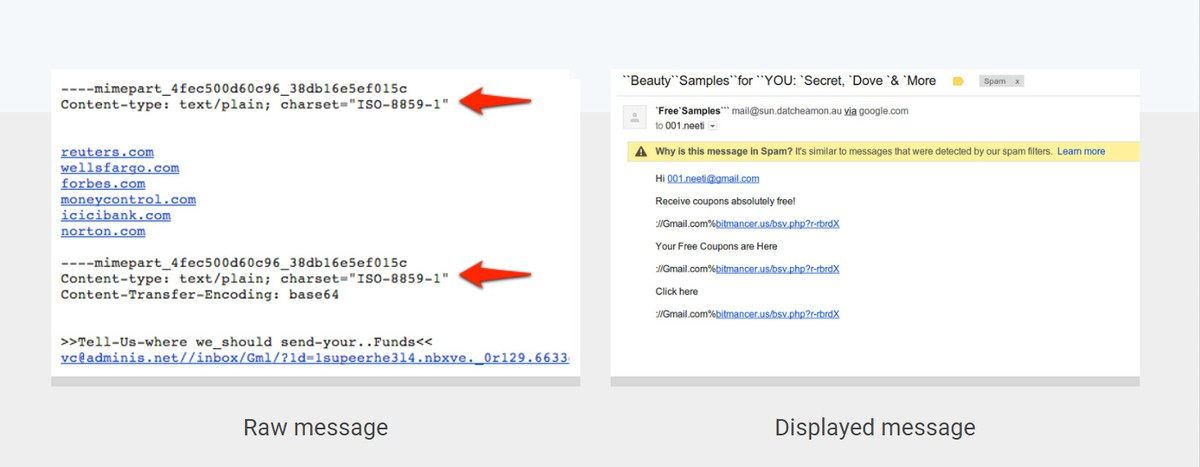
\includegraphics[width=0.45\textwidth,height=6cm]{pictures/1.png}
\begin{center}
Fig 1: Instance of the adversarial i/p
\end{center}

Most generally, classifiers face two types of adverse inputs: altered parameters, that are variations of a recorded threat deliberately crafted that bypass the algorithm, and zero-day parameters which are occasionally visible in-front of the payloads. 
\section{Mutated i/p:}
In recent years, we have noticed an explosion of illicit tools intended to support cyber criminals build invisible payloads that are best known in the shadows as "FUDs" . Such devices range through testing systems that make it possible to check payloads towards with the help of some malware predating soft wares, which can be used to automate the flow of hackers which attempt to inject suspicious information in such a way that makes the hackers untraceable. \\

\newline

\includegraphics[width=0.45\textwidth,height=6cm]{pictures/2..png}
\begin{center}
Fig 2: AVs tester services vs Obfuscator services
\end{center}

It is therefore essential to build up a detection systems in a certain manner that it is difficult for attackers to optimize payloads. Here are three main concept approaches to deal with this.
\section{1.Control the info leak}
The agenda over here is to ensure the intruder obtain very less information as they check the devices. They are necessary inorder to hold input to a minimum and to postpone it at the maximum, e.g. avoid returning specific error codes or trust values.
\section{2. Control probing}
The purpose of such a strategy would be to reduce the  hackers through growing the amount of payloads that can be tested against your computers. By that how much an attacker will operate against your systems, you will every the speed at which malicious payloads are created.\\

\newline
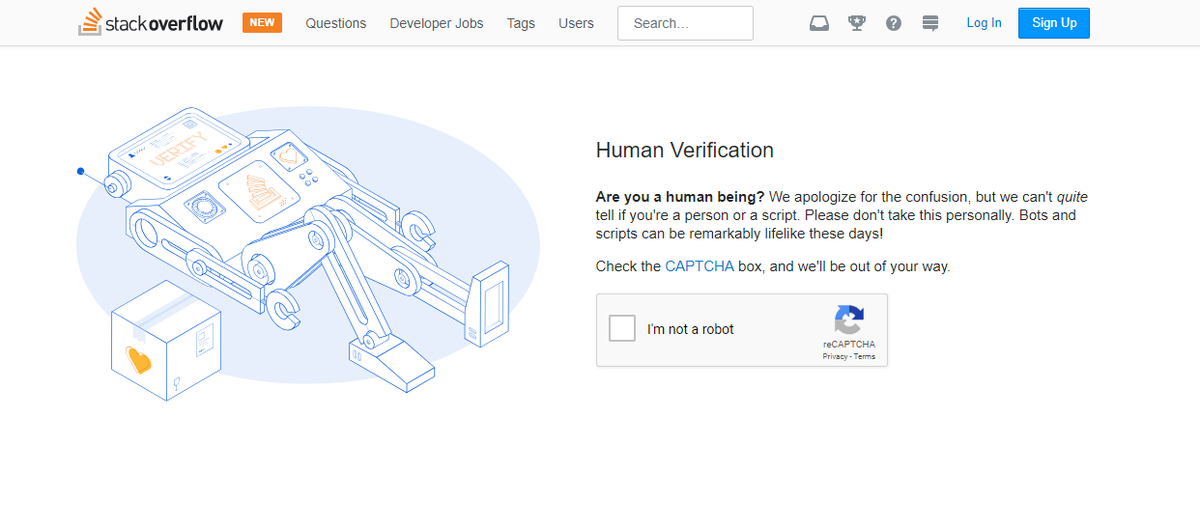
\includegraphics[width=0.45\textwidth,height=6cm]{pictures/3..png}
\begin{center}
Fig 3: Example of such a rate restriction
\end{center}


Such a approach are also applied by enforcing a degree of constraint on finite resources, like the IP and the profiles. The common instance of this frequency constraint is that it helps a user in repairing the CAPTCHA when it is published at all as seen here.
The detrimental issue that this aggressive rating restriction is that it provides an opportunity for poor players to build false accounts and use corrupted consumer machines to diversify their IP pools. The pervasive usage of industry-wide limitations on prices is a significant driving force behind the emergence of very successful dark market platforms where profiles and IP addresses are regularly sold.

\section{ Ensemble learning}
It is therefore necessary to incorporate different prevention strategies that render it more challenging for offenders who exploit your entire program. Using community education to combine specific types of detecting approaches, such Artificial Intelligence  algorithms, classification laws and phenomenon detection, increases the usability of the system as good players can create payloads that will ignore each of these systems at once.\\

\newline
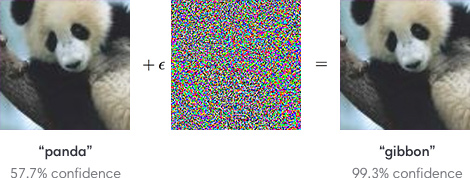
\includegraphics[width=0.45\textwidth,height=6cm]{pictures/4..png}
\begin{center}
Fig 4: Details of adverse attacks on neural networks
\end{center}

We add multiple classifiers and auxiliary systems to ensure Gmail's robustness against spammers. Such methods have a  system,with a very big genetic algorithm which includes deep learning clustering algorithm, and other methods.\\A really ongoing experimental  field was how to create adversarial models which manipulate deep neural networks . Now it is a trick in creating an unnoticeable disturbance which totally tricks deep neural networks, seen in the screen shot above.\\
New analysis reveals how CNN is susceptible towards negative data attacks because it tends towards study simplified database frequency rather than making assumptions  and learning elevated-level description that is somewhat prone to noise.
Such type of attack affects several DNNs. By a defense point of view, this method of assault also shown very troublesome, because it do not really have any efficient means of defending ourselves from these assaults.\\
Essentially, they may not have a reliable method for DNNs to generate a fair values  to all components. Training it to use it is incredibly difficult, because DNNs conduct co-linear / non-convex modifications in quite big places, which would be really need to make them aware on how to exercise elevated-standard description in such a way that it generalizes well. \\


\section{Zero day Attacks:}
New attacks are the other obvious form of adversarial i/p  which can fully disregard classifiers.  Attacks wouldn't occur too much, but it is always necessary to find a way to cope to them because they are catastrophic.
Latest attacks are the obvious method of adversarial variables which can be completely ignored by the algorithms. There are not many new attacks, but it's always essential to find ways to deal with them, as they are often quite dangerous. There are also many possible probable reasons for fresh assaults, in our research, these above two categories of events are likely to trigger them.


\section{feature launch}
By default, introducing features starts a fresh assault surfaces where intruders were very easy in retrieving. This is the reson where it is difficult to have a zero protection day whenever a fresh software is introduced.

\section{Increasing the incentive}
Although seldom mentioned, several modern attacks are powered by a rather lucrative attack vector. If we could notice , it is a clear indication of  increase in abuse of cloud infrastructure. cryptocurrency of reaction  led in a spike in bitcoin prices during the late 2017. When bitcoin values skyrocketed beyond dollars, we noticed a spike in the attacks which was used for snatching Google's cloud storage services from mine.\\
Though, it's not that you can't foresee the assaults are going to throw away your classifier, so whether such an assault is going to hit you're helpless. You should prepare for these attacks to happen and set in motion contingency measures to prevent them. Below are a variety of ways to consider when training for black swan activities.\\

\subsection{Create an accident management protocol:}
The very first step is to develop and review an incident response strategy to insure that you react appropriately once they are  captured  uncontrolled. It includes, which is not restricted in having a correct commands inorderto disrupt and stop execution while checking the lookup tables and knowing whome to be contacted .
The  Site Reliability Engineering Manual which is released by Google should include  disaster management portion and an emergency response segment.Furthermore information on security-related content, is found at the Computer Security Incident Recovery Guide which is released by the National Institute of Standards and Technology..\\
\subsection{Using existence models to defend fresh products:} 
Main challenge that you encounter would be the nonexistence of previous evidence so that you can educate the classifiers. Another approach for tackling the problem would be by using the transition of information, which helps one to leverage learned data from one context and extend it to another.\\
For eg, when dealing with photos, you may use an established pre-trained model, and when  textual cotent comes into picture then we could use common databases for example the Jigsaw data-set.

\section{Flexibile Anomaly Detection}
Anomaly Detection techniques should have been the initial protection line  by definition .An intrusion would produce an unparalleled collection of inconsistencies relating to how the device is abused.
An important example of a innovative assault that caused fresh phenomena was the "MIT casino syndicate" assault on the Massachusetts WinFall lottery game.\\
In 2005, several organizations which was included in the gaming syndicate found  loopholes in the lottery system which was intiated by WinFall. when prize money is shared between the players, you will receive 2.3€ on average for every 2€ ticket you purchased. In order to stop exchanging the winnings with other gangs, the MIT gang planned to carry out a huge purchase of the jackpot tickets 3 weeks before the draw was scheduled. Clearly, the big spike in the draw tickets—purchased by very small personals—started various anomalies found through the gambling groups.\\
Earlier, when bitcoin prices went crazy, we started seeing a group of corrupt individuals trying to take advantage of such a spike in drilling by exploiting Google's database which was set up  for nothing. Inorder to accomplish "simple" situations, they tried to exploit many of the attack vectors that included the effort to abuse our free-tier, the use of stolen payment cards, and the penetration of legitimate cloud consumer computers through phishing. Finally, this type of attack was so popular that millions of people who watched YouTube videos on how to mine . Clearly, we can't imagine that coercive mining is going to be such a major issue.\\
Fortunately, as this happened, we had an incident detection system in place for Cloud storage cases. When expected, as shown in the aforementioned map, that was taken straight through the object detection framework , this points out that when extraction starts, its sequential activity shifts dramatically as the corresponding asset utilization becomes fundamentally different from the traditional resource usage exhibited uncompromised cloud occasions.

\section{Poisoning of the Data}
The second type of attacks encountered by the classifiers relates to opponents seeking to manipulate the data in order to misbehave the program.
\subsection{Model skewing}
Beginning form of attack is known as model skewing, where the intruders contaminate trained values to change the trained boundary between what the classifier classifies as good input and what the classifier classifies as poor input. For eg, model skewing may be used to try to pollute training data to manipulate the classifier to classify unique malicious binaries as benign.

\subsection{Concrete example}
The very initial method of poison assault is named as the model skewing, whereby attackers try to feed the polluted training data in order to alter the learned boundary over what the classifiers classifies with better inputs and what the classifier classifies as bad input. For eg, model skewing can be utilized to seek and contaminate raw data and exploit the classifier and identify particular harmful binaries as harmless.

\subsection{Mitigation strategies}
You should use the following three techniques to keep attackers from skewing models:
Using sensitive data's sampling methods: all we have to guarantee at least specific number of the people, like IP's or the consumers, couldn't compensate with an significant percentage for a model trained results. In the particular, has to cautious not to overweight fake positive and fake negatives has to be identified by the humans.\\
It would theoretically become accomplished by the reducing the amount of instances each and every individual could add, or by utilizing decreasing the weights on depending on about the number of instances recorded.\\
Comparing the recently qualified classifiers' with the least ones to determine on what amount has improved. For an eg, you may execute the darker start and by the comparing all the both two different outputs has be the same traffic. all the alternative solutions including the A / B checking in the percentage of the flow as well as back-testing.\\
Create a gold database for ours classifiers said to be which it has to forecast precisely in order to start development. Ideally, this dataset includes a collection of selected attacks and usual material that is reflective of the program. This method would mean which we could identify whether a weaponizing kind of assault has been abled to produce a very major decline in a model until it said to be adversely impacting the others.

\subsection{Feedback weaponizing Method}
In this second form of the data contamination assault is said to be the hacking of an individuals input mechanisms in order to target legalized users and contents. As long as the perpetrators know that we were utilizing customer reviews, they can seek to use this reality to their benefit in one manner or another — for criminalization purposes.
\subsection{Concrete's examples}
Some of the important significant efforts in order to weaponize consumer reviews, we happen to encountered was in 2017 where it was a grouped community of 4 chained malicious users who wanted that to reclaim the CNN application's ranking in the Google Store and Ios Stores whereby posting thousands of 1-star scores.
Feedbacked devices are being deliberately employed by the bad actors of the variety kind purposes, like trying to knock down the rivals, seeking vengeance, and covering up their tracks.

\subsection{Mitigation strategies}
These were said to be two different main things that has to be bear in our minds when trying to minimize the usage of input: 
do not build a direct correlation of criticism and fines. Instead, before taking a judgment, make sure that the input validity is tested and balanced with other signals.\\
Don't say that the abuser is liable for the material that results from the violence. For eg, it isn't that the video that which has about the hundreds of false likes that which an owner would said to be purchased it. We all 've saw the numerous times whereby criminals have eaten up the law full accurate and genuine material in an effort to hide their traces and or to seek to force us in order to penalise the very innocent individuals or users.

\section{Model-stealing attacks}
The article wouldn't have become finished with no listing assaults aimed at extracting templates or details on a information that is utilized during preparation. These strikes were a major issue as this models contain sensitive intellectual property properties and are based on few of the company's very most important details, such as financialable transactions, health check up records or consumer's payments.\\
making sure of the protection of these models has been trained over the users-specific info, like the cancer related info, was of utmost importance because these models can theoretically be misused to reveal confidential user details.

\section{Attacks}
There are two major model-stealing attacks
\subsubsection{Layout reconstruction}
The main concept here was said to be the intruder is being abeled to replicate a product through searching those publicly available API as well as slowly modifying those own code utilizing it was such as the Oracle. ver most Recently published papers have shown that these assaults tend to get successful against all most on all AI based algorithms.
\subsubsection{Membership leakage}
In this situation, the intruder creates shadow models which allow those to decide if a specified records was utilized in order to train the models. Although these assaults do not recovered the blueprint, they theoretically reveal confidential details.

\section{Categorization of ML threats with respect to defense goals}
Throughout information protection, it is well-established to differentiate between threats throughout terms of their impact on protection objectives. The categorization of reported threats according to defense targets compiles an analysis of clusters with related attack scenarios as well as incomplete yet planned clusters with threats. Such holes in the categorization of attacks that emerge from undisclosed publications concerning attacks on ML elements, unresolved attacks or attacks that have not yet been carried out yet are still imaginable and thus, in theory, observable. Such categorization differences are also especially important. Of special significance for the categorization of the attacks established here is the infringement of the protection objectives that affect the ML variable as a whole. Therefore, violating the dignity of the ML component implies that the ML component itself is modified.\\
A simple peculiarity of ML components relative to conventional applications is their preparation, since there are two main stages in their life cycle: the training process (T) and the delivery period, which we like to term the post-training process (A), since this often calls lifetime learning ML algorithms, which are learned for any feedback even after delivery. A continuous learning approach allows delivery period attacks that are also valid in training time and, on the other hand, disables the applicability of attacks that involve a set target model. Unlike earlier work, we do not determine whether the assault is aimed, whether or not the opponent triggers a certain wrong output, if a wrong output is produced, or if the opponent has awareness of white boxes or black boxes.\\
At this point, too, we are not discriminating between various forms of learning. Given all these kinds of parameters, a blurry categorization will be generated which contradicts a simple differentiation between attacks. Alternatively, we plan to find the above requirements within each of our major categories in order to incorporate more dimensions and to shape sub-groups.\\
Firstly, it can be shown that all assaults during training period harm both credibility and reliability. That actually makes sense immediately: if even the honesty became compromised during the training phase, the device may be modified to conform with the standard by means of the current functionality.\\
Therefore, only a combined assault on all protection targets can be effective during the training process. Confidentiality is not the primary security target of attacks during the training process, but several of the attacks found have often breached confidentiality. However, effective assaults during the training process, which apply exclusively to honesty and durability, may also be conceivable. Attacking protection aim quality makes little sense during the training process. Honesty and stability assaults during the implementation period are technically important and have been reported as necessary. A main category with a relatively high number of reported attacks during the delivery process relates to secrecy. The reality that such assaults are also followed by constraints on availability is more of a side effect than a main factor. A main category with a relatively high number of reported attacks during the delivery process relates to secrecy. The reality that such assaults are also followed by constraints on availability is more of a side effect than a main factor.\\
The lack of attention to the protection principles of honesty and transparency is often especially insightful. In our study, we have not been able to identify any assaults on such protection priorities of the ML elements. Authenticity is typically applied in the environmental aspects of the ML model. This is likely to change in the future, though, with the introduction of robust activities in the ML system network and the need to develop ML components as mission-critical coordination partners. However, we expect whether the new area of attacks on ML components will be opened up in the future in this sector as measures such as the explicable AI (layer-wise distribution of interest, Black Box Explanations by Transparent Approximations, LIME, Generalized Additive Model) and the political need for comprehensible AI decisions would ensure greater comprehensibility.

\section{References}

[1] https://en.wikipedia.org/wiki/Adversarial_machine_learning.

[2] https://www.usenix.org/system/files/conference/usenixsecur\\ity14/sec14-paper-wang-gang.pdf
 
[3] https://www.infoq.com/articles/privacy-attacks-machine-learning-models/.
 
[4] https://towardsdatascience.com/how-to-attack-machine-learning-evasion-poisoning-inference-trojans-backdoors-a7cb5832595c.
 
 [5] https://openai.com/blog/adversarial-example-research/.
 
[6] https://elie.net/blog/ai/attacks-against-machine-learning-an-overview/.
 
[7] https://www.sciencedirect.com/science/article/pii/S15740137\\18303289.
 
[8] http://ceur-ws.org/Vol-2301/paper_2.pdf.
 
[9] https://engineering.virginia.edu/sites/default/files/common/de\\partments/electrical-and-computer-engineering/computer-engineering/files/Threat%20of%20Adversarial%20Attacks.pdf
 
[10] https://yanzzzzz.github.io/files/5040.pdf.
 
[11] https://project.inria.fr/wifs2017/files/2017/12/WIFS_T2_Paper\\not.pdf.
 
[12] https://nvlpubs.nist.gov/nistpubs/ir/2019/NIST.IR.8269-draft.pdf.
 
[13] https://www.cs.cornell.edu/~shmat/shmat_oak17.pdf
 .
[14] https://www.ehidc.org/sites/default/files/resources/files/Ad\\versarial%20attacks%20on%20medical%20machine%20learning.pdf.

[15] https://arxiv.org/ftp/arxiv/papers/1907/1907.07291.pdf.\\


 
\end{thebibliography}
\end{document}
